\documentclass{myproject}

\graphicspath{{../Figures/}}

% title setup
\title{\vspace*{-1cm}Solving the Inviscid Burgers' Equation Numerically}
\date{}
\author{
    Andre Gormann\\
    agormann@sfu.ca
    \and
    Ethan MacDonald\\
    jem21@sfu.ca
}

% bibliography
\addbibresource{references.bib}

\renewcommand*{\thefootnote}{[\arabic{footnote}]}
\newtheorem{theorem}{Theorem}

\begin{document}

% title creation
\maketitle
\vspace*{-1cm}
% contents
\tableofcontents

% document 
\section{Introduction}

The 1-D inviscid Burgers' equation is a first-order hyperbolic partial differential equation (PDE) of the form
\begin{equation}\label{burgers_long}
    \partial_t u(x,t) + u(x,t)\partial_xu(x,t) = 0
\end{equation}
where $u \in C^1(\Omega)$, and $x,t \in \Omega \subset \R\times\R^+$. Note that a more compact form of \eqref{burgers_long} is $u_t + uu_x = 0$. The latter formulation is what is commonly seen in literature. 

This equation has a brother named the \emph{viscous} Burgers' equation (or simply referred to as Burgers' equation), which takes the form
\begin{equation}\label{burgers_viscous}
    u_t + uu_x = \epsilon u_{xx}
\end{equation}
where $\epsilon > 0$ is the diffusion coefficient. We mention this because the inviscid Burgers' equation can be interpreted as resulting from letting $\epsilon \to 0$ in \eqref{burgers_viscous}. This is important because it informs us what the `correct' behavior of \eqref{burgers_long} should be.

The quasilinear equation \eqref{burgers_long} is not the only formulation of the inviscid Burgers' equation, and in a certain sense it is actually the `wrong' one to study. This is because under a few reasonable assumptions, a completely smooth initial profile modeled by \eqref{burgers_long} will devolve into a discontinuous one in finite time. This is unsettling because then \eqref{burgers_long} fails to hold; the partial derivative of a discontinuous function does not exist!

Instead, we rewrite \eqref{burgers_long} as
\begin{equation}\label{burgers_conservative}
    u_t + f(u)_x = 0
\end{equation}
where
\begin{equation}
    f(u) = \frac{1}{2}u^2
\end{equation}
is known as the flux function\footnote{Because the inviscid Burgers' equation can be put into this form, we are able to leverage a whole host of theory concerning advection conservation laws.}. This is known as the conservation form of the inviscid Burgers' equation. If we integrate \eqref{burgers_conservative} over $[a,b]$, where $[a,b] \subset \Omega$, then we get
\begin{equation}\label{burgers_integral}
    \frac{d}{dt}\int_{a}^{b} u(x,t) dx = f(u(a,t)) - f(u(b,t))
\end{equation}
where we have exchanged differentiation and integration. The form \eqref{burgers_integral} is known as the integral form of \eqref{burgers_conservative}, and it is where the `conservative' notion comes from\footnote{A more explicit derivation of \eqref{burgers_integral} can be found in Section 2.1 of \cite{leveque2002}.}.

Importantly, this integral form has no problems admitting profiles $u$ with spatial discontinuities (we assume it is not also discontinuous in time). It is this formulation (along with \eqref{burgers_conservative}) that we will be studying and developing our numerical schemes for, not the quasilinear form. 

\section{Theory}

We will begin by introducing some notation that will be used throughout this section\footnote{The content of this entire section has been primarily adapted from \cite{leveque1992} and \cite{leveque2002}.}. Supposing that $\Omega = [a,b]\times\R^+$, we discretize the interval $[a,b]$ into a vector of $N$ points $x_j$ by defining a fixed mesh-width\footnote{It is possible to use a variable mesh-width, but we have elected not to.} $\Delta x = (b-a)/N$ so that
\begin{equation}
    x_j = a + j\Delta x.
\end{equation}
Note that we are assuming periodic boundary conditions so that $x_0 = x_{N}$, and so we have exactly $N$ points. For reasons that will soon become clear, we are also interested in the half-steps $x_{j\pm1/2}$ defined by
\begin{equation}
    x_{j\pm1/2} = x_j \pm \frac{\Delta x}{2}.
\end{equation}
Time will simply be denoted by $t_n$, with no explicit formula. This is because for stability purposes (see Section 2.4), we require a variable time-step.

We denote the \emph{pointwise values} of the true solution $u$ which solves \eqref{burgers_conservative} exactly at the mesh point $(x_j, t_n)$ by 
\begin{equation}
    u_j^n = u(x_j,t_n).
\end{equation}
The \emph{cell averages} about the mesh point $(x_j, t_n)$ are then defined by
\begin{equation}\label{cell_average}
    \overline{u}_j^n = \frac{1}{\Delta x} \int_{x_{j-1/2}}^{x_{j+1/2}} u(x,t_n) dx.
\end{equation}

\subsection{Finite Volume Methods for Conservation Laws}

For finite difference methods, at each time $t_n$, we are computing a vector $U^n \in \R^N$ where the $j$-th component $U_j^n$ approximates the pointwise true solution $u_j^n$. In light of \eqref{burgers_integral} though, it is perhaps more natural to instead view $U_j^n$ as approximating the \emph{cell average} $\overline{u}_j^n$. This gives rise to what is known as a \emph{finite volume method}.

If we integrate \eqref{burgers_integral} from time $t_n$ to $t_{n+1}$, we get
\begin{align}
    \int_{x_{j-1/2}}^{x_{j+1/2}} u(x,t_{n+1}) dx = &\int_{x_{j-1/2}}^{x_{j+1/2}} u(x,t_{n}) dx \nonumber \\
    &- \left[ \int_{t_n}^{t_{n+1}} f(u(x_{j+1/2},t)) dt - \int_{t_n}^{t_{n+1}} f(u(x_{j-1/2},t)) dt \right].
\end{align}
Dividing by $\Delta x$ and applying \eqref{cell_average} yields
\begin{equation}
    \overline{u}_j^{n+1} = \overline{u}_j^n - \frac{1}{\Delta x}\left[ \int_{t_n}^{t_{n+1}} f(u(x_{j+1/2},t)) dt - \int_{t_n}^{t_{n+1}} f(u(x_{j-1/2},t)) dt \right].
\end{equation}

The goal of a successful finite volume method then is to accurately model the flux through the boundaries of each cell. Explicitly, we want to find some numerical flux function $\mathcal{F}$ so that 
\begin{align}
    \mathcal{F}(U_j^n, U_{j+1}^n) &\approx \frac{1}{\Delta t} \int_{t_n}^{t_{n+1}} f(u(x_{j+1/2}, t)) dt \\
    \mathcal{F}(U_{j-1}^n, U_{j}^n) &\approx \frac{1}{\Delta t} \int_{t_n}^{t_{n+1}} f(u(x_{j-1/2}, t)) dt.
\end{align}

To this end, we say that a numerical method is in \emph{conservation form} if 
\begin{equation}\label{conservation_form}
    U_j^{n+1} = U_j^n - \frac{\Delta t}{\Delta x} \left[ \mathcal{F}(U_{j}^{n}, U_{j+1}^{n}) - \mathcal{F}(U_{j-1}^{n}, U_{j}^{n}) \right].
\end{equation}
Note that while this derivation comes about through the introduction of control volumes, we can also understand it through the lens of finite differences. Specifically, from \eqref{burgers_conservative} we get the relation
\begin{equation}
    \frac{U_j^{n+1} - U_j^n}{\Delta t} + \frac{F_{j+1/2}^n - F_{j-1/2}^n}{\Delta x} = 0
\end{equation}
where $F_{j\pm1/2}^n \sim \mathcal{F}$ as before.

\subsection{The REA Algorithm and Godunov's Method}

The reconstruct-evolve-average (REA) algorithm is characterized by the following three-step process:
\begin{enumerate}
    \item
    First we \emph{reconstruct} a piecewise polynomial function $p(x,t_n)$ from the approximate cell averages $U_j^n$. Though we will be only considering piecewise linear polynomials, there is no explicit limit on the degree of these $p$.

    \item
    Using the $p(x,t_n)$ as initial data, we then \emph{evolve} the PDE until time $t_{n+1}$ into the future.

    \item
    Finally, we \emph{average} the updated polynomial over each grid cell, obtaining new approximate cell averages
    \begin{equation}
        U_j^{n+1} = \frac{1}{\Delta x} \int_{x_{j-1/2}}^{x_{j+1/2}} p(x,t_{n+1}) dx.
    \end{equation}
\end{enumerate}

For the basic Godunov method, we employ piecewise-constant polynomials $p(x,t_n)$. We say basic, because it is possible to obtain higher-order accuracy by utilizing piecewise-linear polynomials. Due to the added complexity, we will not be exploring this any further. The numerical flux function $\mathcal{F}$ is defined by
\begin{equation}
    \mathcal{F}(u_L, u_R) = \begin{cases}
        \min_{u \in [u_L,u_R]} f(u) \qquad & u_L \leq u_R \\
        \max_{u \in [u_R,u_L]} f(u) \qquad & u_L > u_R 
    \end{cases}
\end{equation}
The notation $u_L$ and $u_R$ will become more clear in the next section. 

\subsection{The Riemann Problem and Managing Discontinuous Solutions}
A Riemann problem is an initial value problem (IVP) for a conservation equation where the supplied initial profile consists of piecewise constant data with a single discontinuity. Typically, the discontinuity is located at $x=0$, so that the initial data is of the form
\begin{equation}
    u(x,0) = \begin{cases}
        u_L \qquad & x < 0 \\
        u_R \qquad & x \geq 0
    \end{cases}
\end{equation}
This problem is very important for the inviscid Burgers' equation specifically because for those points sufficiently away from the discontinuity, we can solve it exactly via the method of characteristics (see Appendix A.2). How we resolve those points near the discontinuity is a bit more complicated. One can appeal to the Lax entropy condition\footnote{See \cite{leveque2002}, Section 11.2 for more information.} which states that, for the inviscid Burgers' equation, a discontinuity propagating with speed $s$ is valid if $u_L > u_R$ (see Figure 1a). The exact speed of this discontinuity, referred to as a shock, is determined by the Rankine-Hugoniot condition\footnote{See \cite{leveque2002}, Section 11.8 for a derivation.}, which for the inviscid Burgers' equation is simply $s = (u_L + u_R)/2$. The solution to this problem is then
\begin{equation}\label{shockwave}
    u(x,t) = \begin{cases}
        u_L \qquad & x < st \\
        u_R \qquad & x \geq st
    \end{cases}
\end{equation}

Alternatively, one may recall that \eqref{burgers_long} can be interpreted as the inviscid limit of Burgers' equation. By admitting a small, but nonzero, $\epsilon > 0$, one can study the behavior near a discontinuity. This is formally known as the vanishing-viscosity approach. By doing so experimentally, the Lax entropy condition is corroborated and the profile \eqref{shockwave} is seen. Moreover, the vanishing-viscosity approach reveals the correct behavior when $u_L < u_R$; a rarefaction wave (see Figure 1b). 
\begin{equation}
    u(x,t) = \begin{cases}
        u_L \qquad & x < u_Lt \\
        x/t \qquad & u_Lt \leq x \leq u_Rt \\
        u_R \qquad & x > u_Rt
    \end{cases}
\end{equation}





\begin{comment}
\begin{equation}
    F(u_L, u_R) = \begin{cases}
        f(u_L) \qquad &s \geq 0 \\
        f(u_R) \qquad &s < 0
    \end{cases}
\end{equation}


\end{comment}







\begin{figure}
    \centering
    \begin{subfigure}{.48\textwidth}
        \centering
        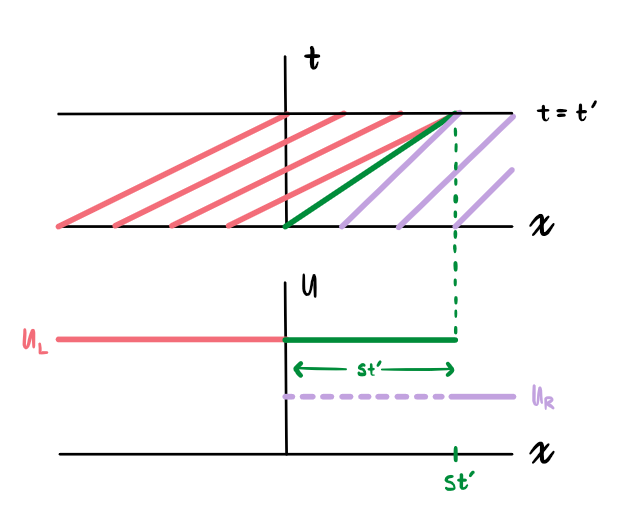
\includegraphics[width=1.0\textwidth]{riemann_shockwave.png}
        \caption{Resolution of a Riemann problem when $u_L > u_R > 0$. A shockwave propagates to the right with speed $(u_L+u_R)/2$.}
        \label{fig:shock}
    \end{subfigure}\hfill
    \begin{subfigure}{.48\textwidth}
        \centering
        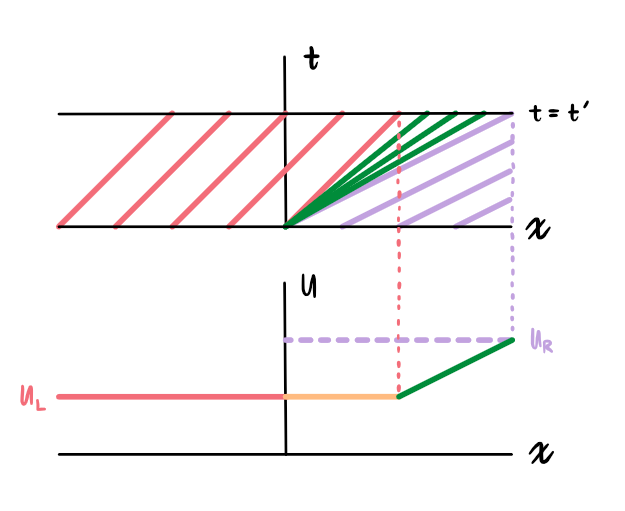
\includegraphics[width=1\textwidth]{riemann_rarefaction.png}
        \caption{Resolution of a Riemann problem when $0<u_L<u_R$. A rarefaction wave fills the void left by the characteristics.}
        \label{fig:rarefaction}
    \end{subfigure}
    \caption{Resolving the discontinuity in a Riemann problem.}
    \label{fig:riemann_discontinuities}
\end{figure}

\subsection{Convergence Notions}

We wish to develop what it means for some approximate cell averages $U_j^n$ to converge to a weak solution $u$ of \eqref{burgers_integral}. To this end, we define a piecewise-constant function $U^{(\Delta t)}(x,t)$\footnote{It is unclear what is gained by this definition as by construction $U^{(\Delta t)}$ agrees with $U_j^n$.} by
\begin{equation}
    U^{(\Delta t)}(x,t) = U_j^n \qquad (x,t) \in [x_{j-1/2}, x_{j+1/2}) \times [t_n, t_{n+1})
\end{equation}
Now since weak solutions are not unique, we define the set
\begin{equation}
    \mathcal{W} = \{u : u(x,t) \text{ is a weak solution to \eqref{burgers_integral}}\}
\end{equation}
Then the global error\footnote{The $w \in \mathcal{W}$ feels like a typo. Due to our unfamiliarity with the material though, we will leave it as printed in \cite{leveque2002}, p. 246.} is given by
\begin{equation}
    \text{dist}\left(U^{(\Delta t)}, \mathcal{W}\right) = \inf_{w \in \mathcal{W}} \| U^{(\Delta t)} - u \|_{1,T}
\end{equation}
where 
\begin{equation}
    \|v\|_{1,T} = \int_{0}^{T} \|v(\cdot,t)\|_1dt = \int_{0}^{T}\int_{\R}|v(x,t)|dx dt
\end{equation}
Lastly, we define the total variation of a collection of cell averages $U^n$ by 
\begin{equation}
    \text{TV}(U^n) = \sum_{j=1}^N |U_j^n - U_{j-1}^n|
\end{equation}
We are now ready to state the convergence result.
\begin{theorem}
    Suppose $U^{(\Delta t)}$ is generated by a numerical method in conservation form with a Lipschitz continuous numerical flux, consistent with some scalar conservation law. If the total variation $TV(U^n)$ is uniformly bounded for all $n$, $\Delta t$ with $\Delta t < \Delta t_0$, $n \Delta t \leq T$, then the method is convergent in the sense that the global error $\text{dist}\left(U^{(\Delta t)}, \mathcal{W}\right) \to 0$ as $\Delta t \to 0$.
\end{theorem}
In the paper \cite{leveque1985}, the necessary conditions are proven to hold for the Godunov method, and so we have formal verification that our method is convergent\footnote{While we would have liked to prove some of this ourselves (or at the very least explain the result more thoroughly), the material is simply too advanced for us.}. One of the assumptions made though is that either of the following CFL conditions are satisfied
\begin{equation}
    \max_{j} |U_j^n| \frac{\Delta t_n}{\Delta x} \leq \frac{1}{2} \qquad \text{or} \qquad \max_{j} |U_j^n| \frac{\Delta t_n}{\Delta x} \leq 1
\end{equation}
The latter has the property that solutions to neighboring Riemann problems may interact. \Cite{leveque1985}, argues that this is not a problem though, and experimentally we have verified this (see Section 3).
\begin{comment}
\subsubsection{Numerical Convergence}

With the intent of redeeming ourselves for our poor understanding of the analytic material, we present some ideas for verifying convergence numerically. Because of the piecewise-constant construction of the cell averages $U_j^n$, we have that Godunov's method is at most first order accurate in space. We will verify this experimentally in Section 3 with our test problems by means of mesh-refinement: at fixed grid cells, we will compare the differences 


have verified this experimentally on regions where the profile $u$ is smooth; the difference in accuracy between two mesh-sizes varies with order $\Delta x$. At points near or at the discontinuities though, the results are observed to be more chaotic (which makes sense; a small perturbation in time or space can cause a large difference), and so we cannot really compare accuracy. 
\end{comment}


\section{Experiments}

We will be verifying our theory experimentally on five different problems. The first two are Riemann problems which are `easy' in the sense that a MATH student familiar with the relevant material should be able to characterize the solution completely. The consequence of this is that we can hard-code the solutions to compare against with respect to accuracy, both for our methods and for the Physics Informed Neural Network (PINN).

In contrast, we are unable to resolve the `hard' problems analytically and so cannot directly compute the accuracy of our methods. Instead, we will have to employ numerical convergence studies and rely on the soundness of the underlying theory.

\subsection{`Easy' Problems}

\subsubsection{Riemann problem: shockwave}

The initial value problem (IVP) of interest is
\begin{equation}\label{IVP:shock}
    \begin{cases}
        u_t + uu_x = 0 \quad x \in (-\pi,\pi), \: t > 0 \\
        u(-\pi,t) = 1 \\
        u(\pi,t) = 0 \\
        u(x,0) = u_0(x)
    \end{cases} 
\end{equation}
where 
\begin{equation}
    u_0(x) = \begin{cases}
        1 \qquad & x < 0 \\
        0 \qquad & x \geq 0
    \end{cases}
\end{equation}

Following our prior discussion, the analytical solution is characterized by a shockwave, and is given by
\begin{equation}
    u(x,t) = \begin{cases}
        1 \qquad & x < t/2 \\
        0 \qquad & x \geq t/2
    \end{cases}
\end{equation}
For this problem, we attempted both a numerical approach and a PINN approach. The numerical solution was highly accurate and required little time to compute even when using 1000 grid points. Some plots are shown below.

\begin{figure}
\centering
    \begin{subfigure}{.48\textwidth}
        \centering
        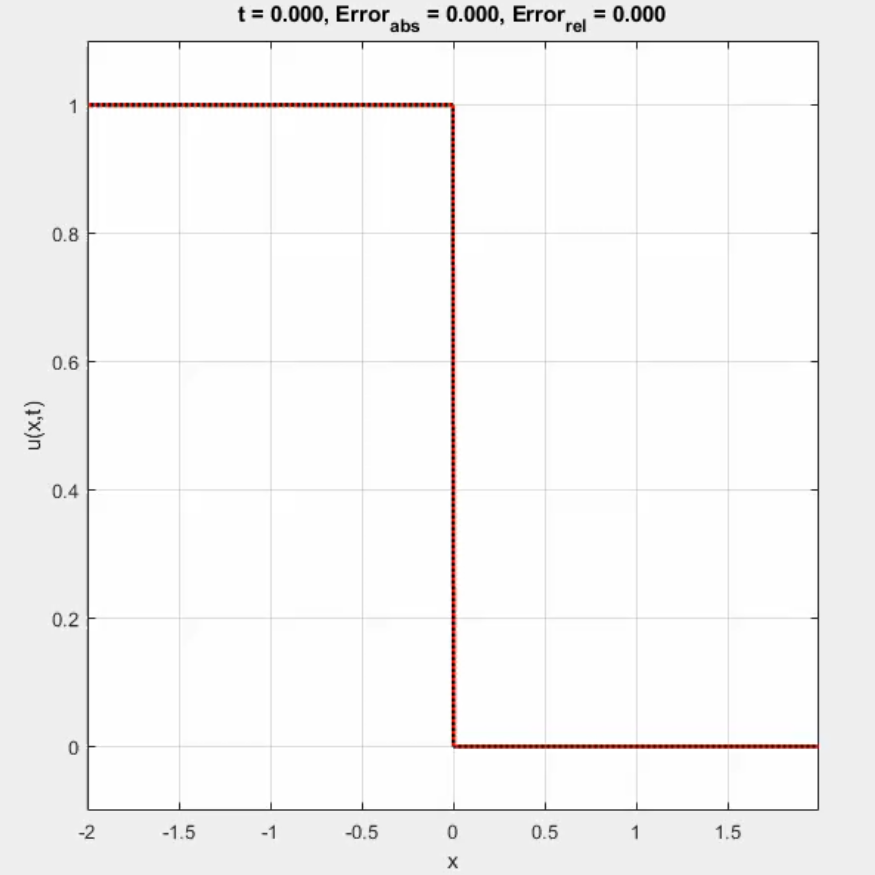
\includegraphics[width=1.0\textwidth]{t0_shockwave.png}
        \caption{Initial state for the Riemann Problem.}
    \end{subfigure}\hfill
    \begin{subfigure}{.48\textwidth}
        \centering
        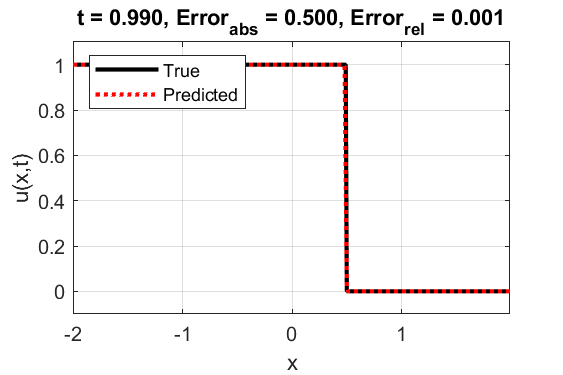
\includegraphics[width=1\textwidth]{t05_shockwave.png}
        \caption{As $t$ increases, the error is small and consistent.}
    \end{subfigure}
    \caption{The numerical solution of the shockwave Riemann problem.}
\end{figure}

When using the PINN approach, we acheived decent results. However, these results are far worse than the numerical solution and took much longer to compute as they required training a neural network. Our neural network used 9 layers with 20 neurons at each layer, as well as 10 000 internal collocation points during training. The code used for the PINN approach in this problem and the next were adapted from the MathWorks example ``Solve PDE Using Physics-Informed Neural Network.'' Some plots are shown below.

\begin{figure}
\centering
    \begin{subfigure}{.48\textwidth}
        \centering
        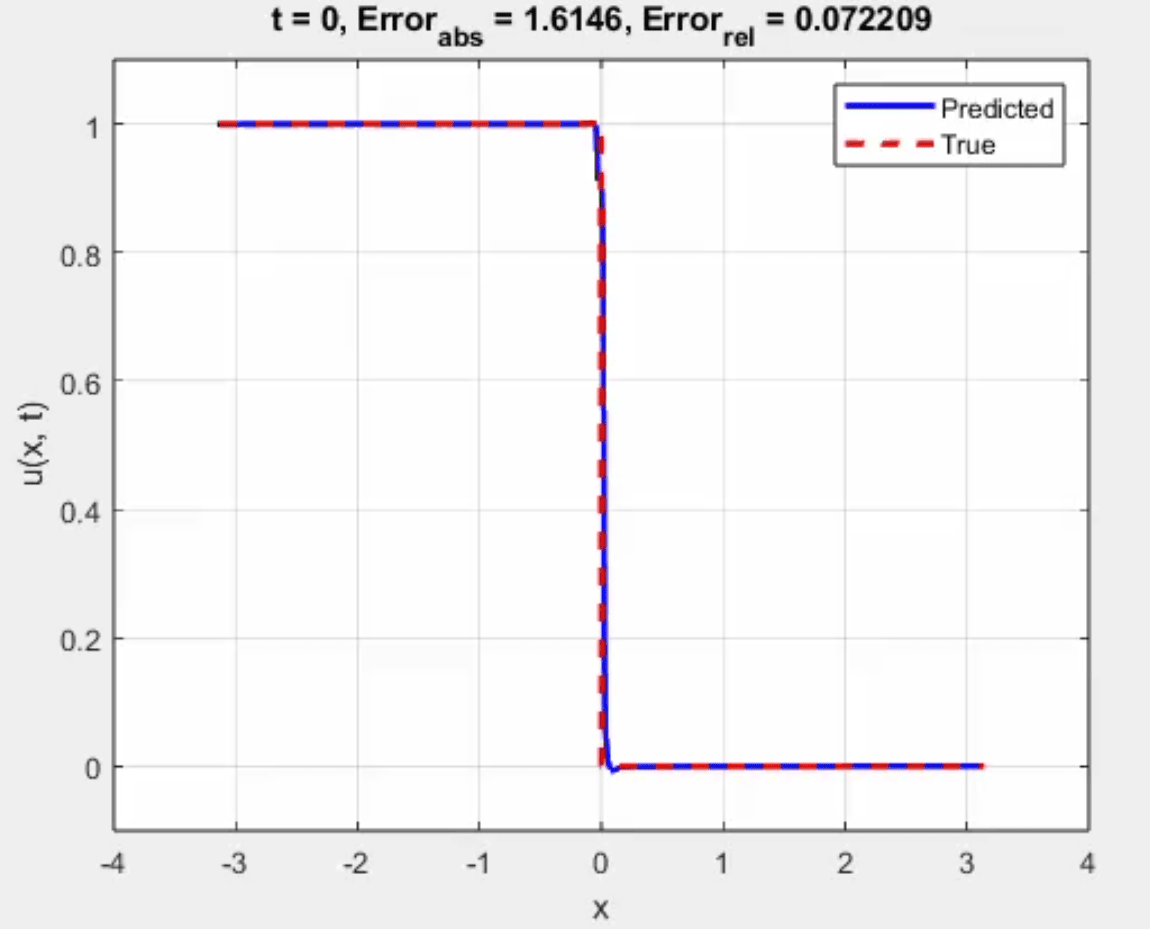
\includegraphics[width=1.0\textwidth]{t0_NN_shockwave.png}
        \caption{Initial state. Notice that the neural network cannot acheive perfect accuracy at $t=0$.}
    \end{subfigure}\hfill
    \begin{subfigure}{.48\textwidth}
        \centering
        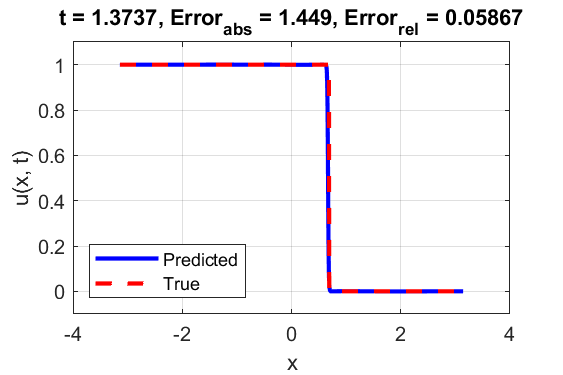
\includegraphics[width=1\textwidth]{t137_NN_shockwave.png}
        \caption{As $t$ increases, the error is larger than in the numerical solution, but still consistent.}
    \end{subfigure}
    \caption{The PINN of the shockwave Riemann problem.}
\end{figure}

\subsubsection{Riemann problem: rarefaction wave}

We modify the \eqref{IVP:shock} slightly so that its solution exhibits a rarefaction fan
\begin{equation}\label{IVP:rarefaction}
    \begin{cases}
        u_t + uu_x = 0 \quad x \in (-\pi,\pi), \: t > 0 \\
        u(-\pi,t) = 0 \\
        u(\pi,t) = 1 \\
        u(x,0) = u_0(x)
    \end{cases} 
\end{equation}
where 
\begin{equation}
    u_0(x) = \begin{cases}
        0 \qquad & x < 0 \\
        1 \qquad & x \geq 0
    \end{cases}
\end{equation}

Instead of a shockwave, the analytical solution is characterized by a rarefaction wave, and is given by
\begin{equation}
    u(x,t) = \begin{cases}
        0 \qquad & x < 0 \\
        x/t \qquad & 0 \leq x \leq t \\
        1 \qquad & x > t
    \end{cases}
\end{equation}

Once again, we attempted both a numerical approach and a PINN approach. Once again, the numerical approach was fast, accurate, and consistent. Some plots are shown below.


\begin{figure}
\centering
    \begin{subfigure}{.48\textwidth}
        \centering
        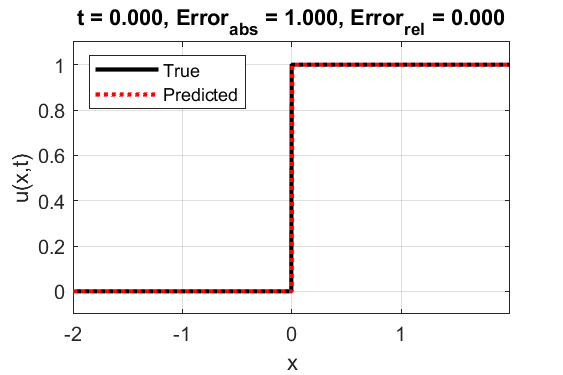
\includegraphics[width=1.0\textwidth]{t0_rarefraction.png}
        \caption{Initial state of the Riemann problem.}
    \end{subfigure}\hfill
    \begin{subfigure}{.48\textwidth}
        \centering
        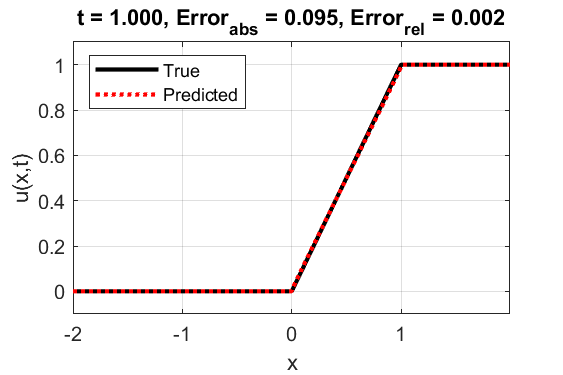
\includegraphics[width=1\textwidth]{t1_rarefraction.png}
        \caption{idk lol}
    \end{subfigure}
    \caption{The numerical solution of the rarefraction wave Riemann problem.}
\end{figure}

When using a PINN approach, the solution is somewhat oscillatory at the steep gradient around $t=0$. However, as time progresses, this oscillation seems to dissipate. We presume that the neural network struggles with the steeper gradients near $t=0$ because the gradient of $u$ is computed as a part of the loss during training. Naturally, this becomes less of a problem as $t$ increases because the gradient becomes more shallow and changes at a slower rate. The PINN solution can also be seen lagging behind the true solution. Presumably, this is a result of the changing gradient and would no longer be an issue for $t \rightarrow \infty $. Some plots are shown below.

\begin{figure}
\centering
    \begin{subfigure}{.48\textwidth}
        \centering
        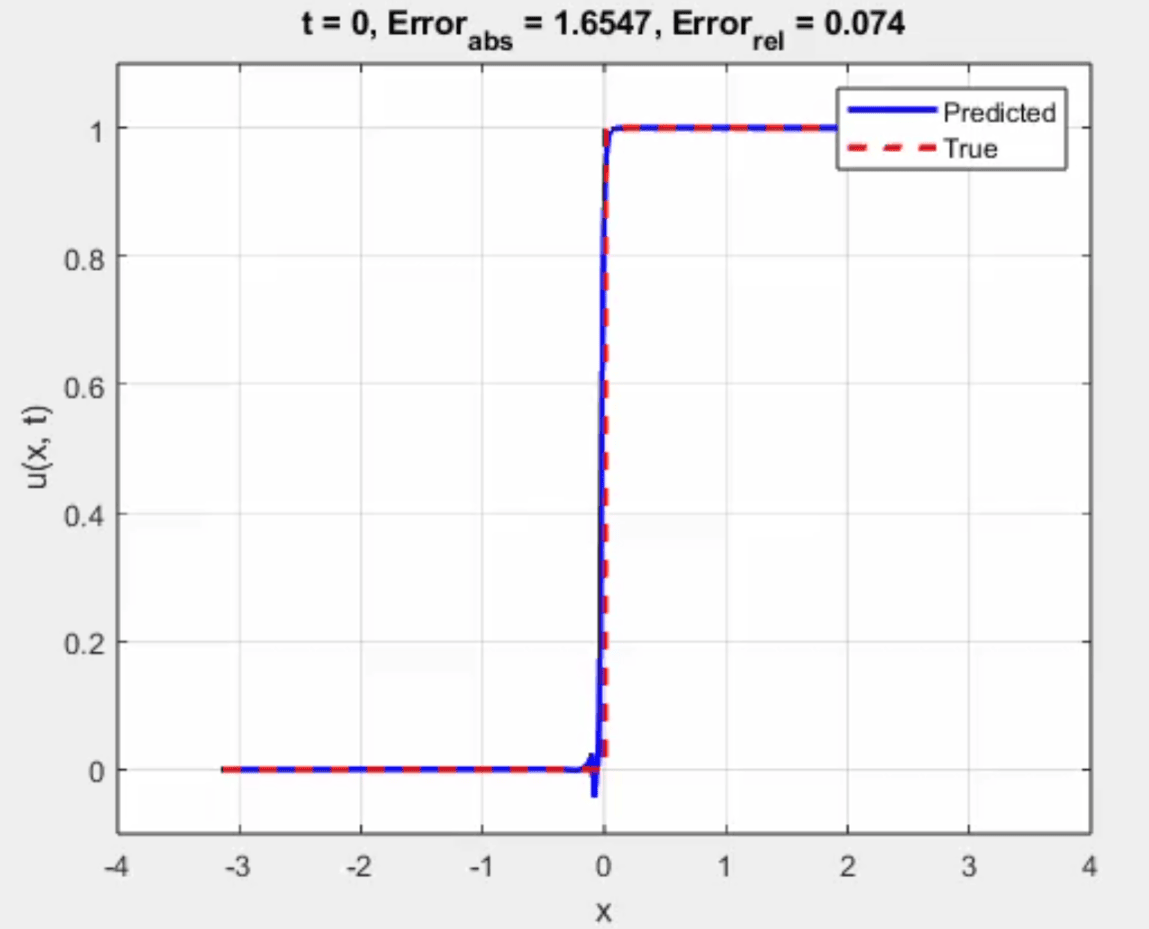
\includegraphics[width=1.0\textwidth]{t0_NN_rarefraction.png}
        \caption{Initial state. Notice that a small oscillation is already being exhibited in $u_L$.}
    \end{subfigure}\hfill
    \begin{subfigure}{.48\textwidth}
        \centering
        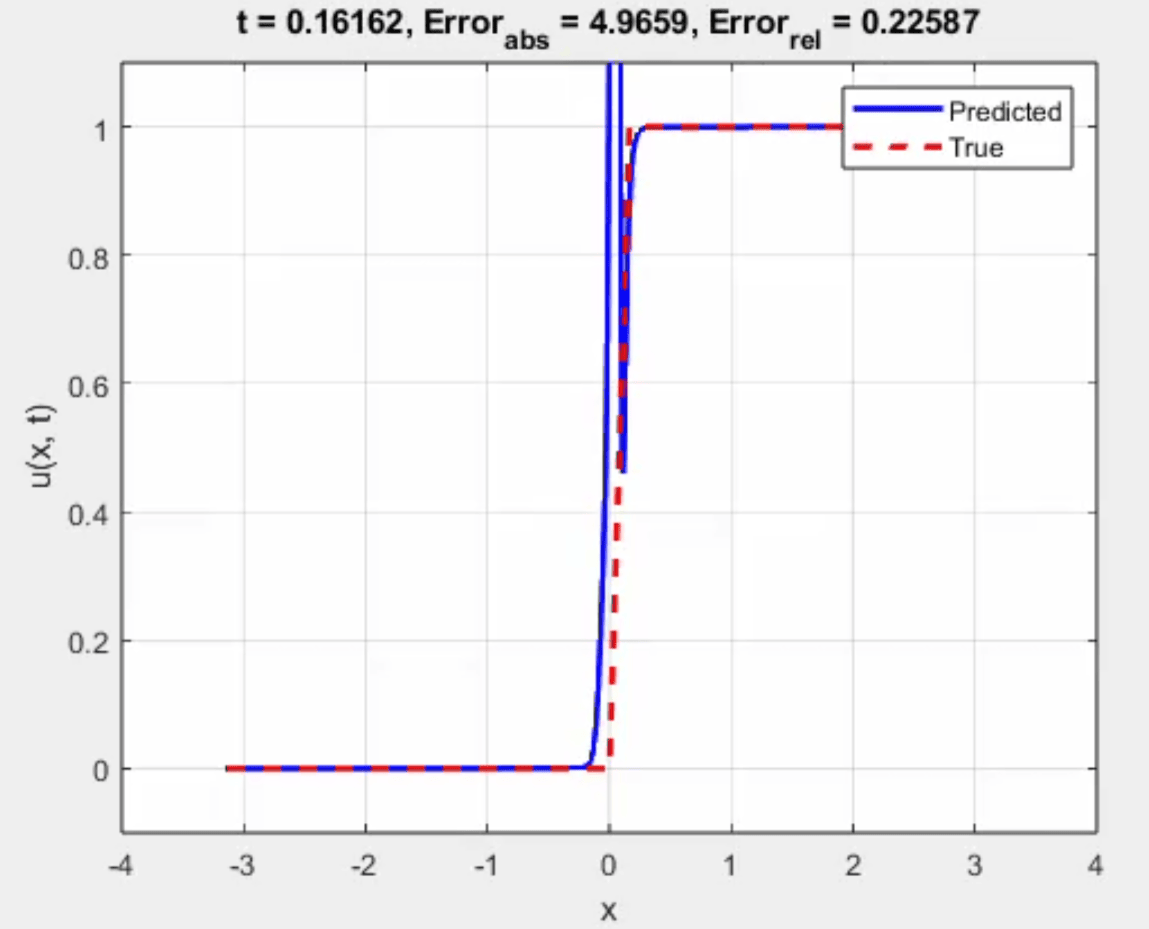
\includegraphics[width=1\textwidth]{t016_NN_rarefraction.png}
        \caption{The oscillation becomes extreme as the gradient changes rapidly.}
    \end{subfigure}
    \begin{subfigure}{.48\textwidth}
        \centering
        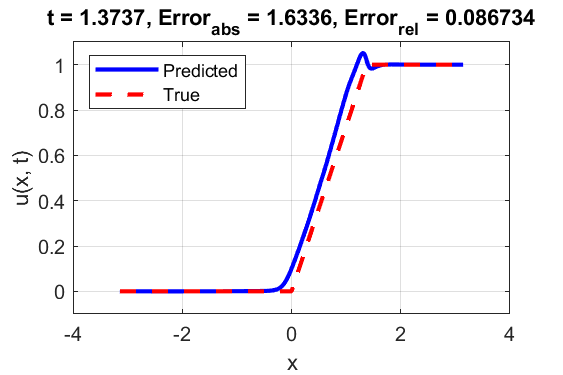
\includegraphics[width=1\textwidth]{t137_NN_rarefraction.png}
        \caption{The oscillation subsides and the PINN solution lags behind the true solution.}
    \end{subfigure}
    \caption{The PINN solution of the rarefraction wave Riemann problem.}
\end{figure}








\subsection{`Hard' Problems}
Snapshots of the results from the numerical solver can be found in Appendix A.1 (we ran out of space in the main document).
\subsubsection{Square wave}

Our first IVP has the form
\begin{equation}\label{square_wave}
    \begin{cases}
        u_t + uu_x = 0, \quad x \in [0, 2\pi], \: t>0 \\
        u(x,0) = u_0(x) \\
        u(0,t) = u(2\pi,t), \quad t > 0
    \end{cases}
\end{equation}
where
\begin{equation}
    u_0(x) = 
    \begin{cases}
        1 \qquad &  x \in [\pi/2, 3\pi/2] \\
        0 \qquad & \text{otherwise} 
    \end{cases}
\end{equation}

 The solution consists of a shockwave propagating to the right along with a rarefaction wave trailing behind. As time elapses, the rarefaction wave eventually catches up to the shock wave and the profile devolves into a sawtooth wave. While it is not possible to compare this solution to an analytical one, we have varied the number of grid cells in an attempt to measure convergence. We certainly see no spurious phenomena, so we can be confident that our solution is accurate to \emph{some} weak solution.

\subsubsection{Sine wave}

The IVP is given by
\begin{equation}\label{sine_wave}
    \begin{cases}
        u_t + uu_x = 0, \quad x \in [0, 2\pi], \: t>0 \\
        u(x,0) = \sin(x) \\
        u(0,t) = u(2\pi,t), \quad t > 0
    \end{cases}
\end{equation}

The solution consists of a stationary shockwave. This is because the initial profile is symmetric and so the shock speed propagating to the right (from the positive profile), and the shock speed propagating to the left (from the negative profile), cancel out. The initial profile converges to a weak solution.

\subsubsection{Sine-squared wave}

We modify the prior IVP slightly
\begin{equation}\label{sine-squared_wave}
    \begin{cases}
        u_t + uu_x = 0, \quad x \in [0, 2\pi], \: t>0 \\
        u(x,0) = \sin^2(x) \\
        u(0,t) = u(2\pi,t), \quad t > 0
    \end{cases}
\end{equation}

The solution consists of shockwaves propagating to the right with rarefaction waves trailing behind. The initial profile converges to a weak solution.

\section{Phyisics Informed Neural Network Scheme}

While a PINN approach worked decently for 

\section{Conclusion}

this shit was way harder than i thought it would be

\newpage
\appendix
\section{Appendix}
\subsection{Figures}

\subsubsection{`Hard' Problems}

\begin{figure}[h]
    \centering
    \begin{subfigure}[b]{0.40\textwidth}
       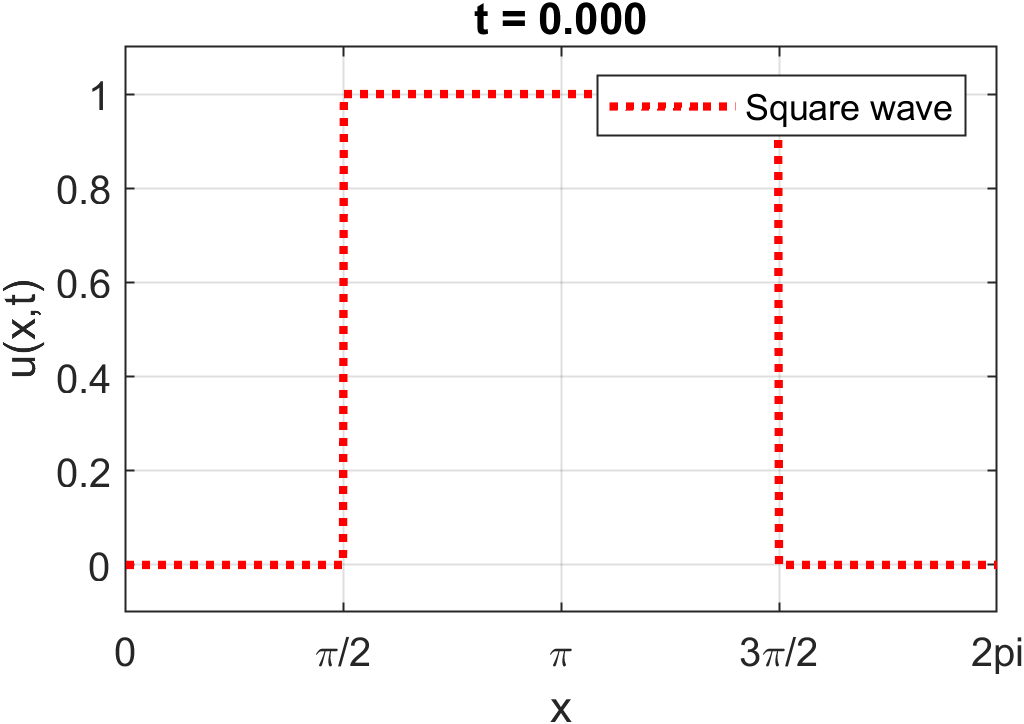
\includegraphics[width=1\linewidth]{square_wave_0.png}
       \caption{}
    \end{subfigure}\qquad
    \begin{subfigure}[b]{0.40\textwidth}
       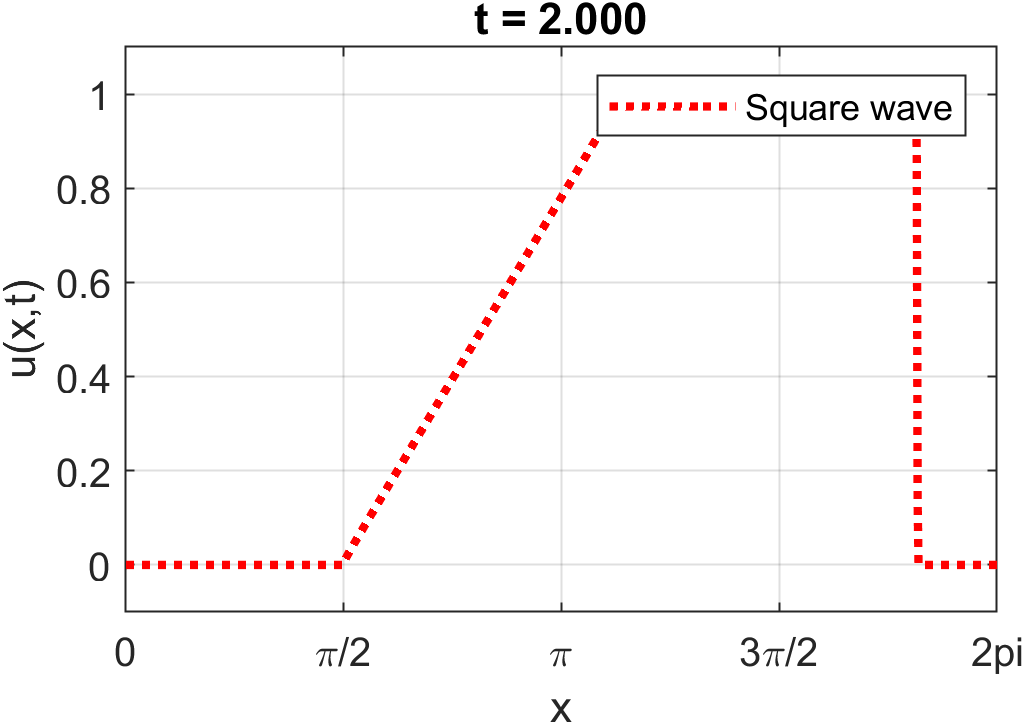
\includegraphics[width=1\linewidth]{square_wave_2.png}
       \caption{}
    \end{subfigure}

    \vspace{\floatsep}

    \begin{subfigure}[b]{0.40\textwidth}
       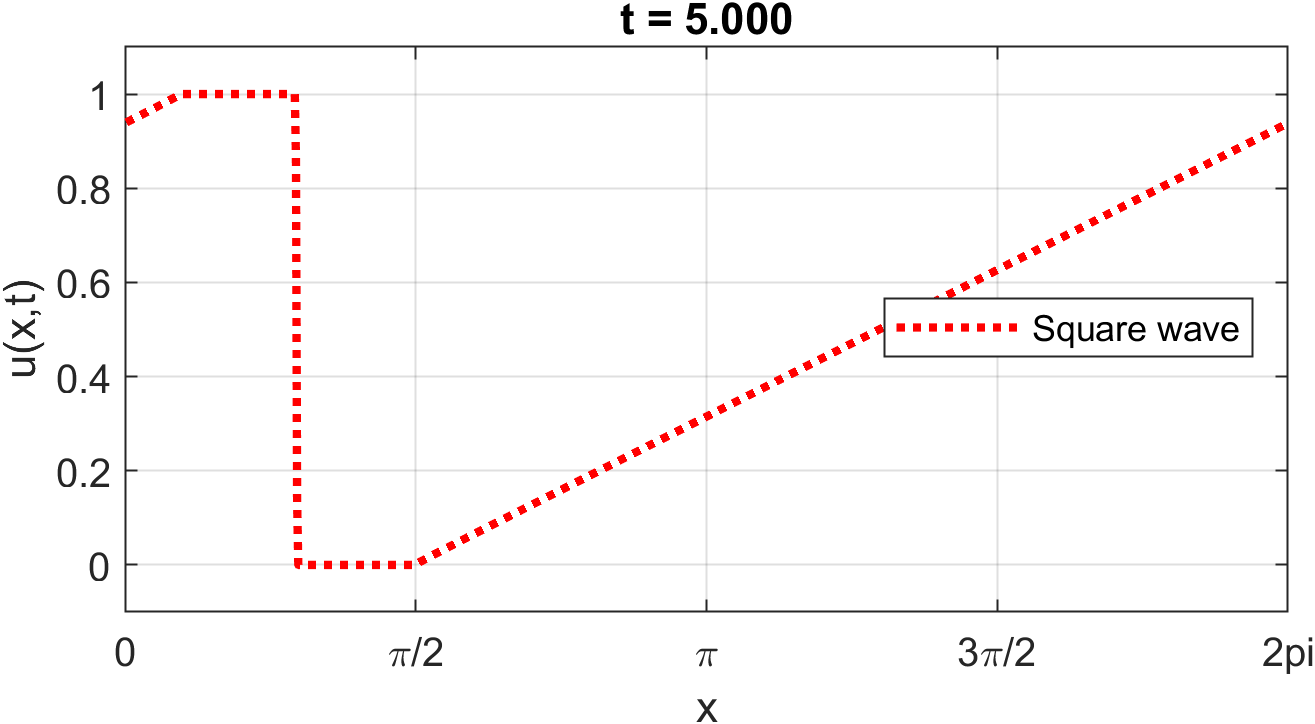
\includegraphics[width=1\linewidth]{square_wave_5.png}
       \caption{}
    \end{subfigure}\qquad
    \begin{subfigure}[b]{0.40\textwidth}
       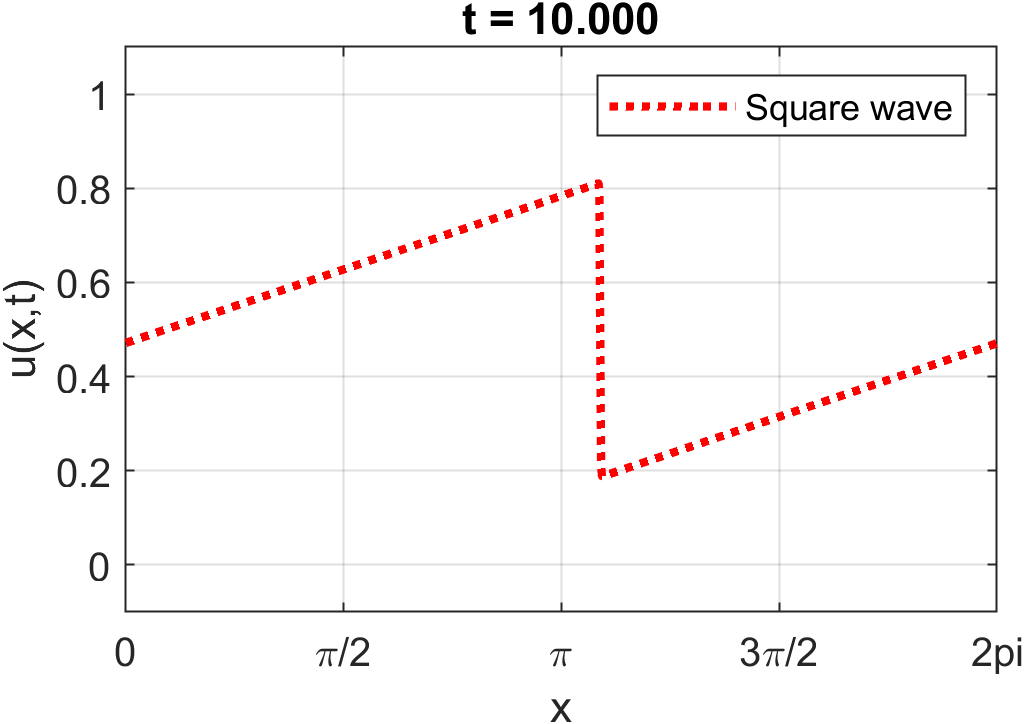
\includegraphics[width=1\linewidth]{square_wave_10.png}
       \caption{}
    \end{subfigure}
    \caption{Numerical solutions to problem \eqref{square_wave}. Snapshots are taken at times $t = 0, 2, 5, 10$.}
\end{figure}

\begin{figure}
    \centering
    \begin{subfigure}[b]{0.40\textwidth}
       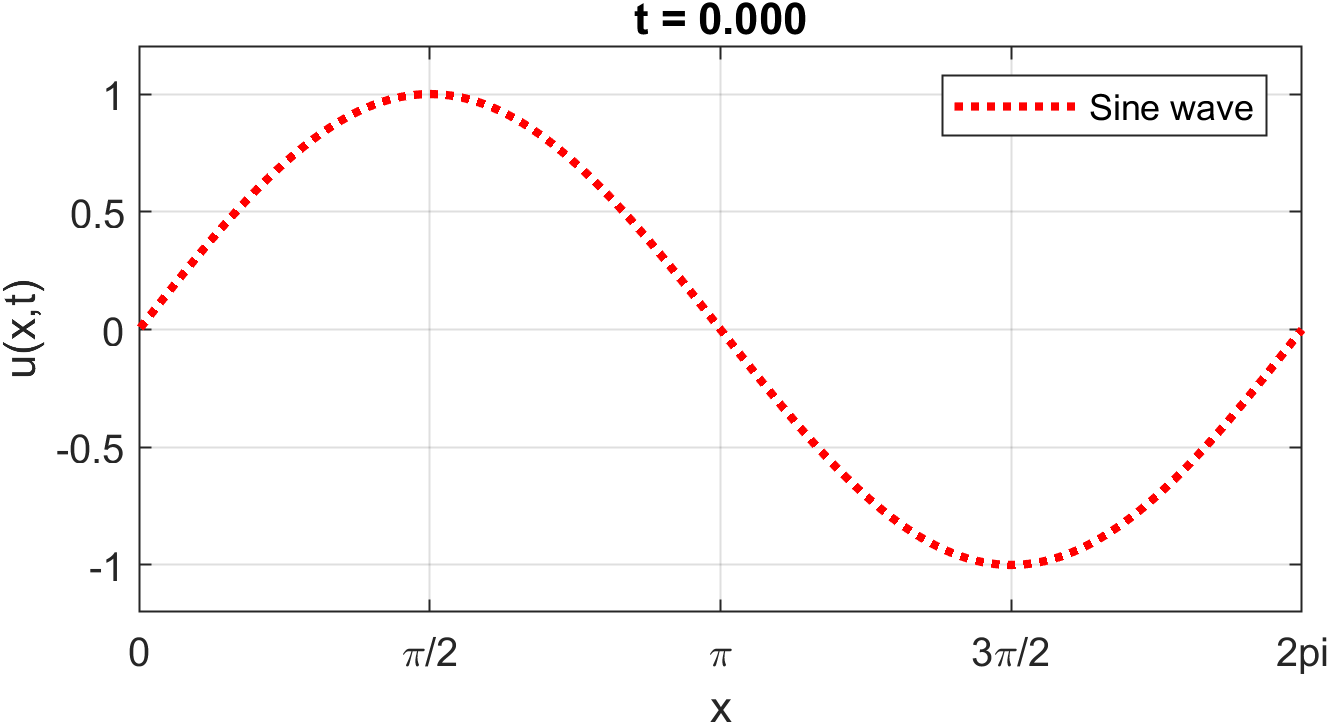
\includegraphics[width=1\linewidth]{sine_wave_0.png}
       \caption{}
    \end{subfigure}\qquad
    \begin{subfigure}[b]{0.40\textwidth}
       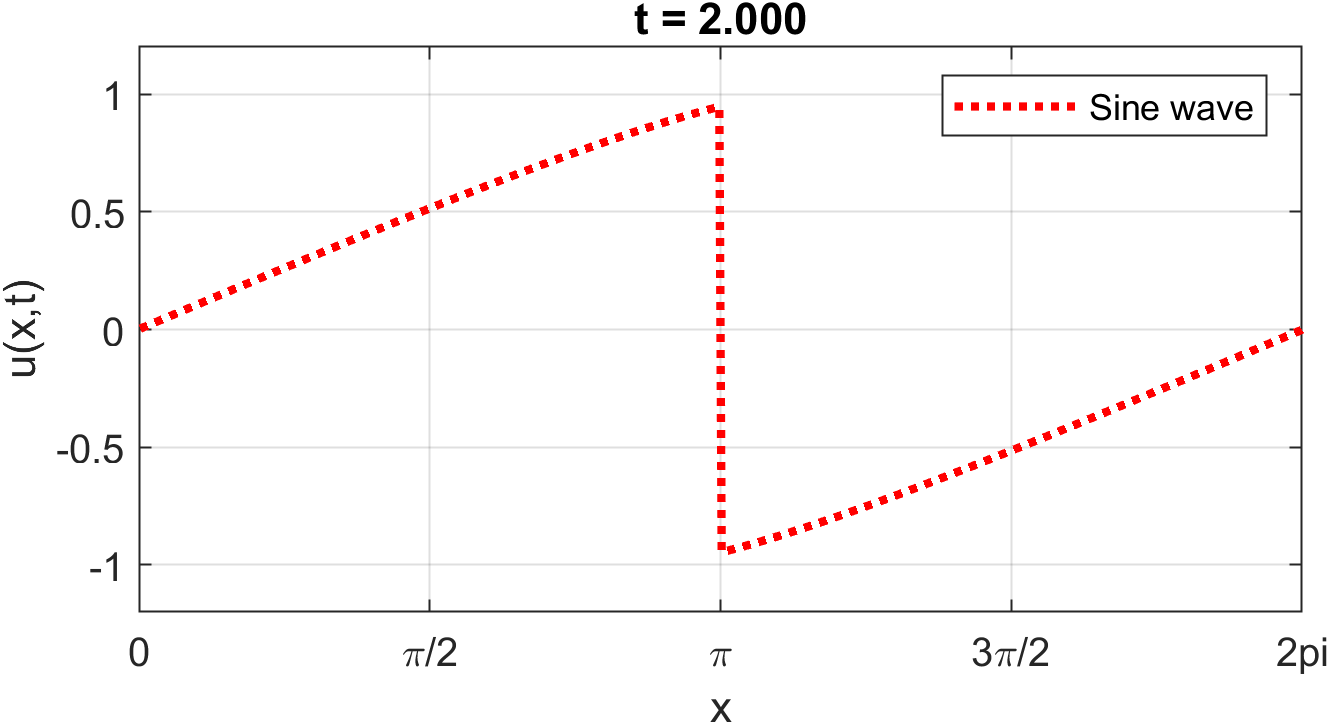
\includegraphics[width=1\linewidth]{sine_wave_2.png}
       \caption{}
    \end{subfigure}

    \vspace{\floatsep}

    \begin{subfigure}[b]{0.40\textwidth}
       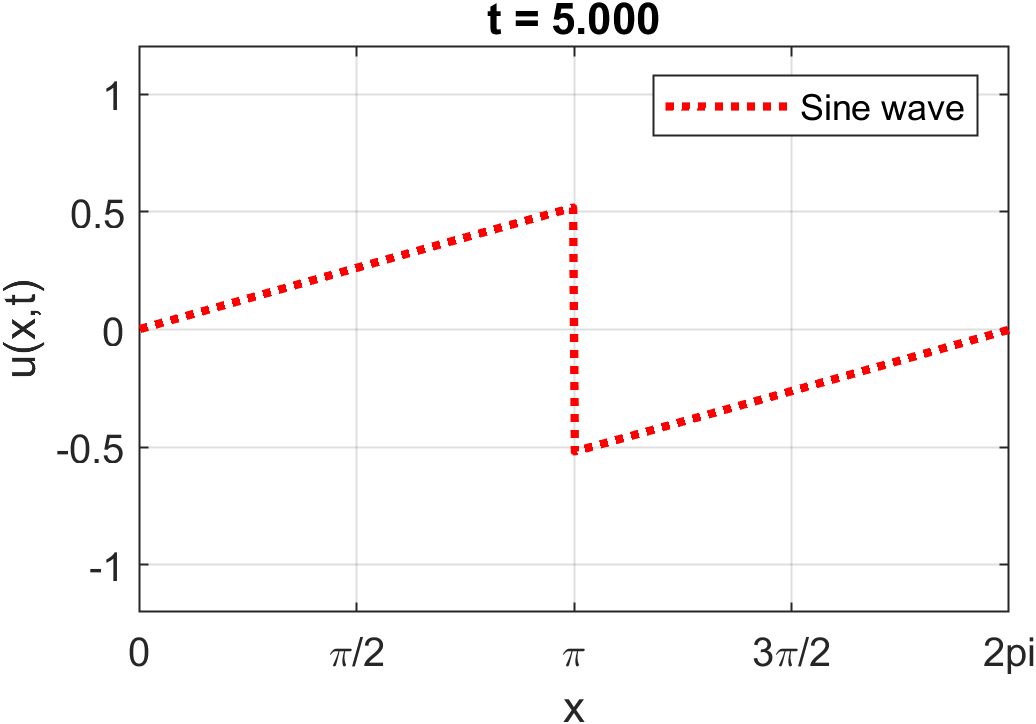
\includegraphics[width=1\linewidth]{sine_wave_5.png}
       \caption{}
    \end{subfigure}\qquad
    \begin{subfigure}[b]{0.40\textwidth}
       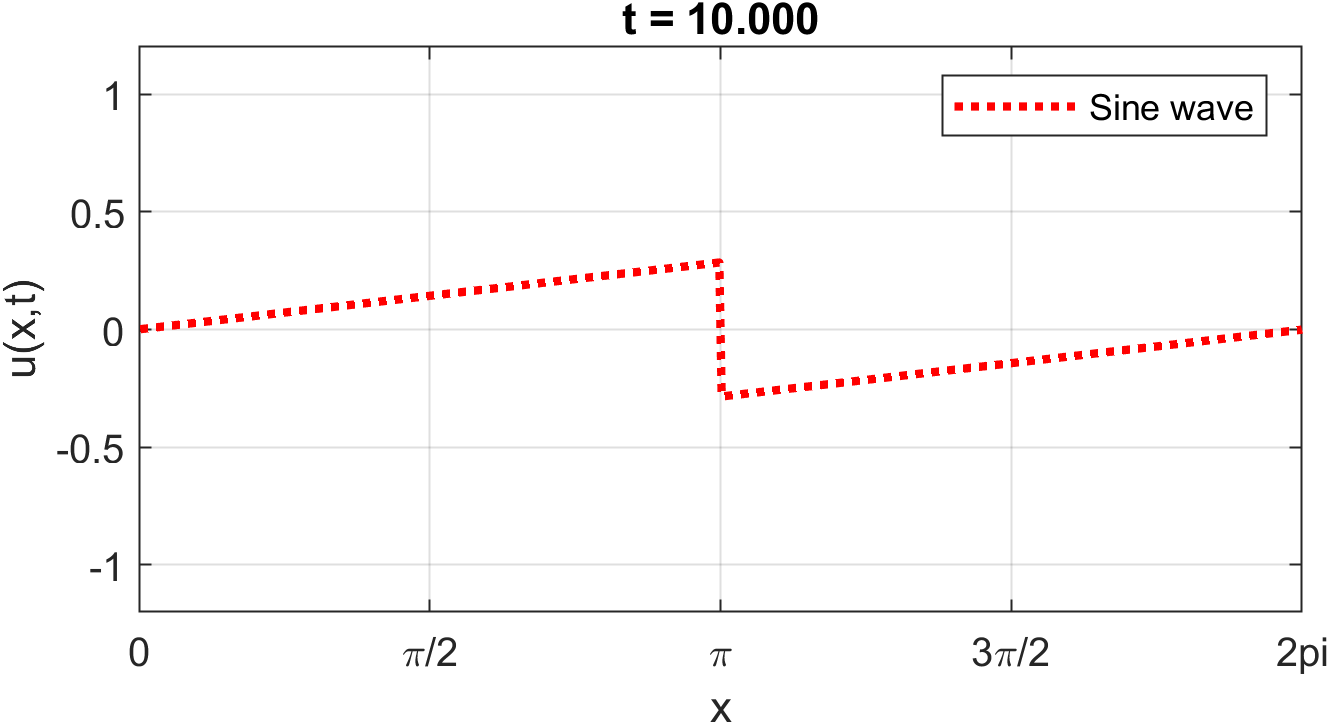
\includegraphics[width=1\linewidth]{sine_wave_10.png}
       \caption{}
    \end{subfigure}
    \caption{Numerical solutions to problem \eqref{sine_wave}. Snapshots are taken at times $t = 0, 2, 5, 10$.}
\end{figure}


\begin{figure}
    \centering
    \begin{subfigure}[b]{0.40\textwidth}
       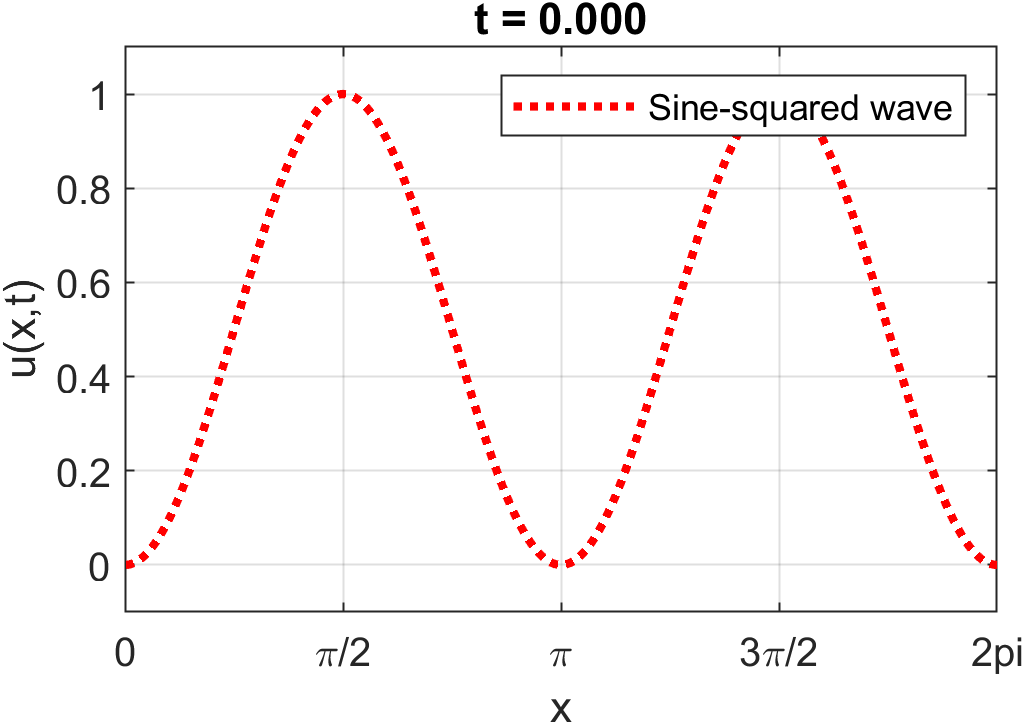
\includegraphics[width=1\linewidth]{sine-squared_wave_0.png}
       \caption{}
    \end{subfigure}\qquad
    \begin{subfigure}[b]{0.40\textwidth}
       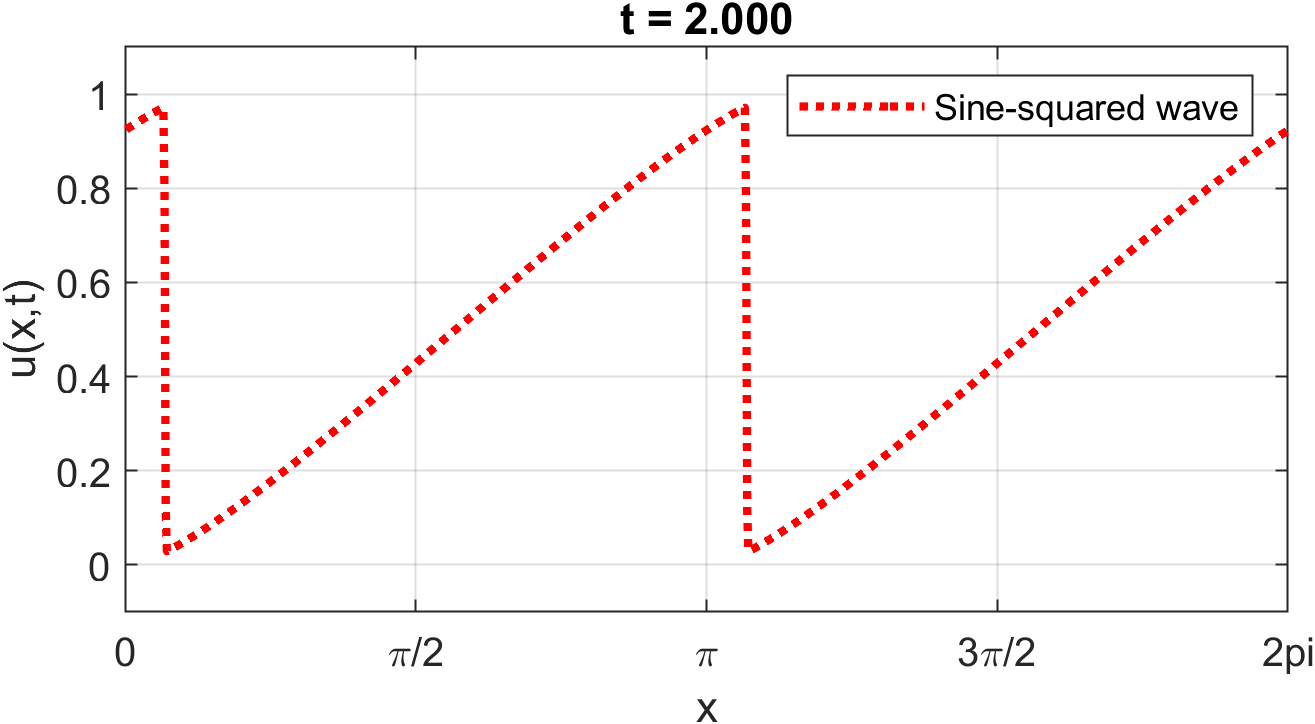
\includegraphics[width=1\linewidth]{sine-squared_wave_2.png}
       \caption{}
    \end{subfigure}

    \vspace{\floatsep}

    \begin{subfigure}[b]{0.40\textwidth}
       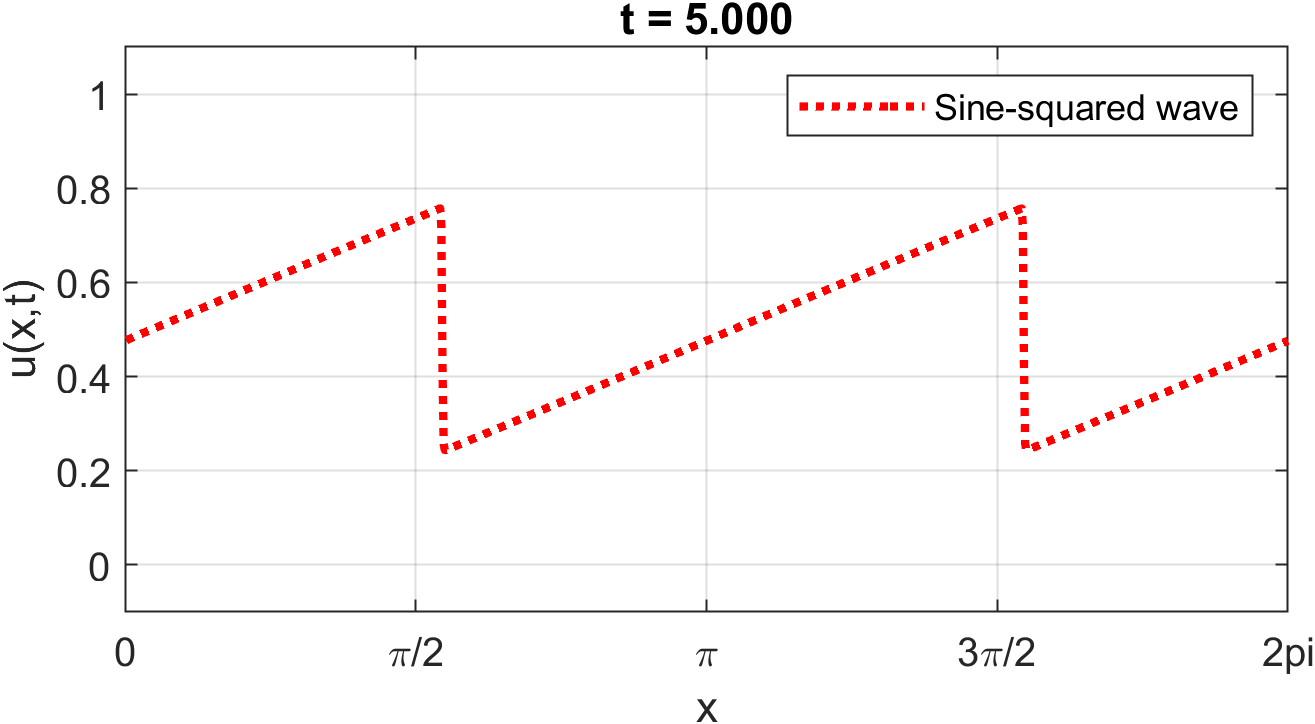
\includegraphics[width=1\linewidth]{sine-squared_wave_5.png}
       \caption{}
    \end{subfigure}\qquad
    \begin{subfigure}[b]{0.40\textwidth}
       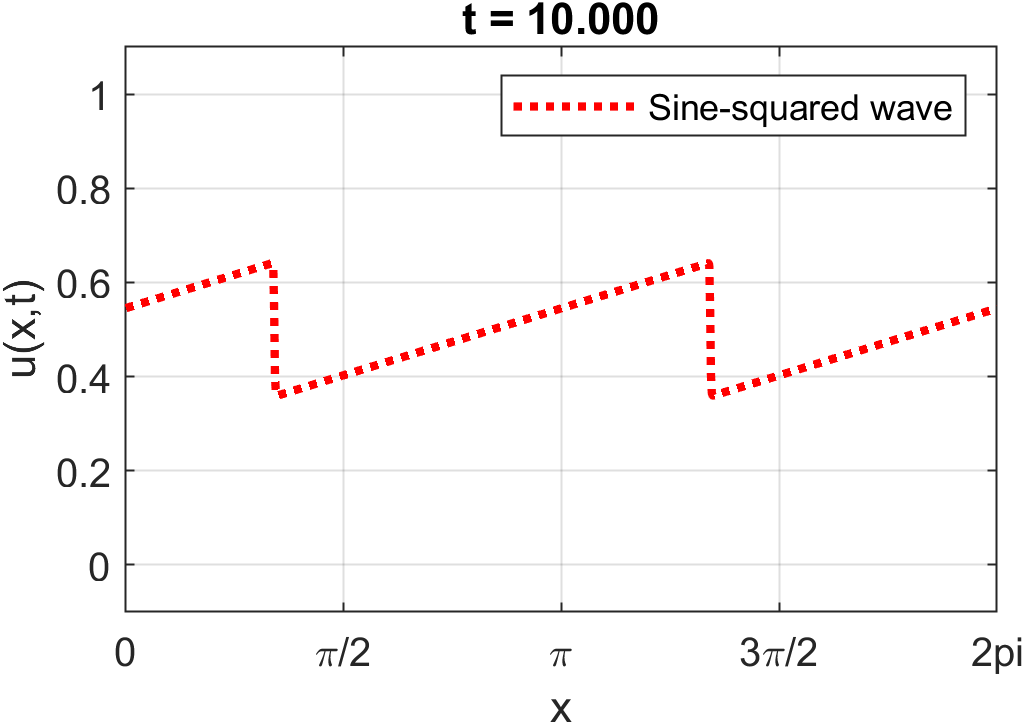
\includegraphics[width=1\linewidth]{sine-squared_wave_10.png}
       \caption{}
    \end{subfigure}
    \caption{Numerical solutions to problem \eqref{sine-squared_wave}. Snapshots are taken at times $t = 0, 2, 5, 10$.}
\end{figure}

\pagebreak
\subsection{Code}

All project code can be found on our GitHub page: \url{https://github.com/agormann/MACM416-project}.
\begin{lstlisting}[
frame=single,
numbers=left,
style=Matlab-Pyglike]
function [T,U] = godunov(X,u0,tf)
%GODUNOV Solves the inviscid burgers equation via the finite volume method.
% Input
%   X := grid of x values
%   u0 := initial profile
%   tf := final time
% Output
%   T := time-steps that the problem was solved at
%   U := profiles at times t in T

% Setup
f = @(u) 0.5*u.^2; % flux function
nx = length(X);
dx = abs(X(1)-X(2));
u = u0;
t = 0;
U = u;
T = t;

% Solution
% dt = dx/max(abs(u)); % fix dt for mesh refinement
while t < tf
    dt = dx/max(abs(u)); % compute dt (dynamic)
    flux = f(u); % initial flux
    F = zeros(size(u)); % flux update
    % solving riemann problem exactly
    for i = 1:nx
        uL = u(i);
        fuL = flux(i);
        uR = u(mod(i,nx)+1);
        fuR = flux(mod(i,nx)+1);
        if uL <= uR
            F(i) = min(fuL,fuR);
        elseif uL > uR
            F(i) = max(fuL,fuR);
        else
            error('OOPSIE WOOPSIE!!')
        end
    end
    u = u - dt/dx*(F - circshift(F,1)); % conservative update
    t = t + dt; U = [U; u]; T = [T; t];
end
end
\end{lstlisting}

\pagebreak
\begin{lstlisting}[
frame=single,
numbers=left,
style=Matlab-Pyglike]
function [T,U] = godunov_dirichlet(X,u0,tf)
%GODUNOV_DIRICHLET Solves the inviscid burgers equation via the finite volume method. 
% Dirichlet boundary conditions are assumed.
% Input
%   X := grid of x values
%   u0 := initial profile
%   tf := final time
% Output
%   T := time-steps that the problem was solved at
%   U := profiles at times t in T

% Setup
f = @(u) 0.5*u.^2; % flux function
nx = length(X);
dx = abs(X(1)-X(2));
u = u0;
t = 0;
U = u;
T = t;

% Solution
while t < tf
    dt = dx/max(abs(u)); % compute dt (dynamic)
    flux = f(u); % initial flux
    F = zeros(size(u)); % flux update
    % solving riemann problem exactly
    for i = 1:nx-1
        uL = u(i);
        fuL = flux(i);
        uR = u(mod(i,nx)+1);
        fuR = flux(mod(i,nx)+1);
        if uL <= uR
            F(i) = min(fuL,fuR);
        elseif uL > uR
            F(i) = max(fuL,fuR);
        else
            error('OOPSIE WOOPSIE!!')
        end
    end
    for i = 2:nx-1
        u(i) = u(i) - dt/dx*(F(i)-F(i-1)); % conservative update
    end
    t = t + dt; U = [U; u]; T = [T; t];
end
end
\end{lstlisting}

\pagebreak
\begin{lstlisting}[
frame=single,
numbers=left,
style=Matlab-Pyglike]
function U = riemann(uL,uR,X,T)
%RIEMANN Solves a riemann problem exactly.
% Input
%   uL := value of profile to the left of 0
%   uR := value of profile to the right of 0
%   X := grid of x values
%   T := specific times to solve the problem at
% Output
%   U := matrix whose rows are the solution to the riemann problem at times specified in T.

nx = length(X);
u0 = uL*(X<0) + uR*(X>=0);

U = [u0; zeros(length(T)-1,nx)];

if uL > uR
    % shockwave
    s = (uL+uR)/2; % rankine-hugoniot condition
    for i = 2:length(T)
        t = T(i);
        U(i,:) = uL*(X<s*t) + uR*(X>=s*t); 
    end
elseif uL < uR
    % rarefaction wave
    for i = 2:length(T)
        t = T(i);
        U(i,:) = uL*(X<uL*t) + (X/t).*((uL*t<=X)&(X<=uR*t)) + uR*(X>uR*t);
    end
end

end
\end{lstlisting}

\pagebreak
\subsection{Analytical Solution via the Method of Characteristics}

We wish to solve the 1-D inviscid Burgers' equation analytically.

Given data on some curve $ \Gamma \subset \overline{\Omega} $, we are looking specific parametric curves $ (x(t), t) $ which connect points $(x, t) \in \Omega$ to $ \Gamma $. We want these curves to be precisely those which are parallel to the vector $(u, 1)$, that is
\[
    \frac{dx}{dt} = \frac{u(x(t), t)}{1} = u(x(t), t)
\]

Now supposing that $u$ solves (2), let $z(t)$ denote the value of $u$ along a characteristic, i.e. 
\[
    z(t) = u(x(t), t)
\]
Then by the chain rule
\[
    \frac{dz}{dt} = \partial_x u(x(t), t) \frac{dx}{dt}u(x(t), t) + \partial_t u(x(t), t)
\]
but $ x'(t) = u(x,t) $, so
\[
    \frac{dz}{dt} = \partial_t u(x(t), t) + u(x,t)\partial_x u(x(t), t)
\]
which is precisely 0 by (2). Hence, we have the following coupled system of ODEs
\begin{equation}
    \begin{cases}
        x'(t) = z(t) = u(x(t), t) \\
        z'(t) = 0
    \end{cases}
\end{equation}
Integrating the second term, we get that
\[
    z(t) = z_0
\]
for some $ z_0 \in \R $. But $z(t) = u(x(t), t)$, so then $u(x(t), t) = z_0$. This corroborates our findings with (3). Now by integrating the first term, we get
\begin{equation}
    x(t) = z_0t + x_0
\end{equation}
where $ x_0 \in \R $. Evaluating at $t=0$, we have that $x(0) = x_0$. Now assuming we are prescribed some initial condition $u(x,0) = g(x)$, we have that (5) becomes
\begin{equation}
    x(t) = g(x_0)t + x_0
\end{equation}
which are exactly those characteristic curves we initially sought.

% bibliography
\nocite{choksi2022}
\nocite{iserles2009}
% \nocite{kutz2013}
% \nocite{trefethen2001}
% \nocite{learncfd}
% \nocite{evans2010}
\nocite{leveque1992}
\nocite{leveque2002}
\printbibliography

\end{document}